\section{Experimental Results}
For our evaluation, we implemented PC extractor module at the 
system call layer 
and PC-Lifetime analyzer and PC-to-Stream mapper module 
at the block device layer in the Linux kernel version 4.5.

In order to evaluate the effectiveness of {\sf PCStream},
we implemented the multi-stream feature and substream concept
to the in-house SSD emulator
based on the open flash development platform~\cite{AMF}.
The number of streams was set to 8 for the evaluation.
The SSD emulator was 12 GB with four channels with four ways, and 
the number of blocks per parallel unit was 512 and
the number of pages per block was 256 with 4KB-sized page.
Due to the limited capacity of the emulator, 
we scaled down the configuration of RocksDB.
The base file size is set to 8 MB
with an 8KB-sized key-value pair and the number of levels was set to 4.
However, the size of level multiplier is remained to be 10 as the general setting,
which means the size of the next level is 10 times larger than the previous level,
to maintain the level access patterns during the compaction.

For benchmarks, we used three scenarios of db\_bench of RocksDB.
The update random scenario (read-modify-write for random keys), {\tt UR}, and 
the append random scenario (read-modify-write with growing values), {\tt AR}, are
for intensively updating key-value pairs.
For each scenario, about 900,000 keys are inserted.
The fill random scenario (write values in random key order), {\tt FR}, 
inserts 300,000 key-value pairs 
after 70\% of the device capacity was filled.

For the comparison, 
we also implemented Autostream, manual technique, and
baseline which does not use the stream allocation policy.
We compared WAF of the existing techniques with {\sf PCStream}
for each scenario and the result is shown in Fig.~\ref{fig:result_emul}. 
We also evaluate the {\sf PCStream} without the second phase stream
assignment to see the effectiveness PC-based data separation, 
denoted by {\sf PCStream--}.

\begin{figure}[t]
	\centering
	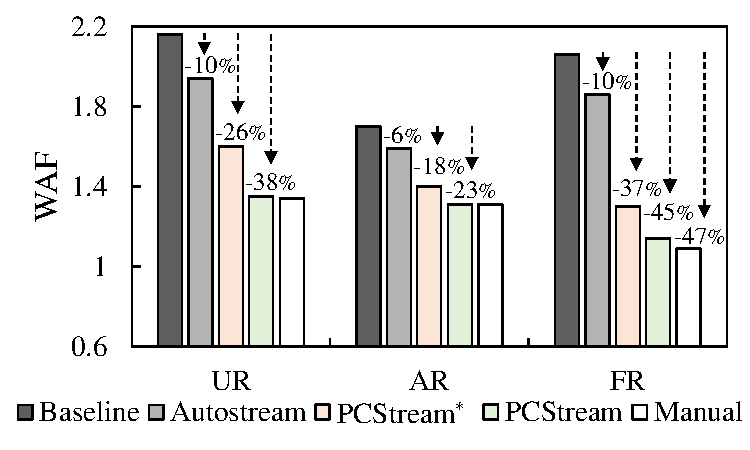
\includegraphics[width=0.8\linewidth]{figure/result_emul}
	\vspace{-10pt}
	\caption{The WAF comparison on the emulator.}
	\label{fig:result_emul}
	\vspace{-15pt}
\end{figure}

As shown in Fig.~\ref{fig:result_emul}, 
{\sf PCStream--} reduces WAF by up to 30\% and by 20\% on average
over the AutoStream. 
The result shows that separating short-lived data such as log or flush
using PC was quite effectvive in reducing WAF.
Moreover, {\sf PCStream} showed similar WAF to the manual technique,
while reducing WAF by up to 38\% and by 30\% on average
over the AutoStream.
The additional benefit comes from separating
long-lived data of compaction during the
second phase assignment.

In order to evaluate the feasibility of {\sf PCStream} on a real SSD,
we used Samsung PM963 480GB SSD (with 8 streams).
As a warming workload, we wrote a single file sequentially to fill 90\%
of logical device capacity, to ensure that 90\% of logical space stays valid
throughout the test.

\begin{figure}[t]
	\centering
	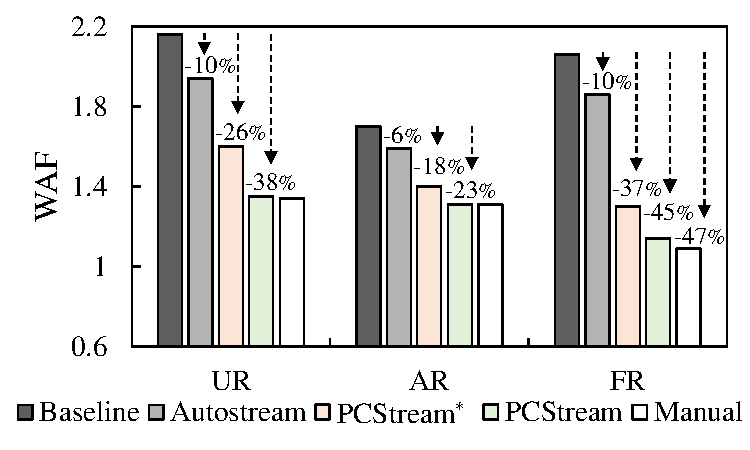
\includegraphics[width=0.8\linewidth]{figure/result_emul}
	\vspace{-10pt}
	\caption{The WAF comparison on the SSD.(temporarily placed to check paper length)}
	\label{fig:result_SSD}
	\vspace{-15pt}
\end{figure}

\vspace{5cm}
\textcolor{blue}{Space for explaining the result on the real SSD.}
\vspace{5cm}
